\documentclass[tikz,border=5pt]{standalone}
\usepackage{pgfplots}
\usepackage{xcolor}
\pgfplotsset{compat=newest}

\pagecolor{white}

\begin{document}

    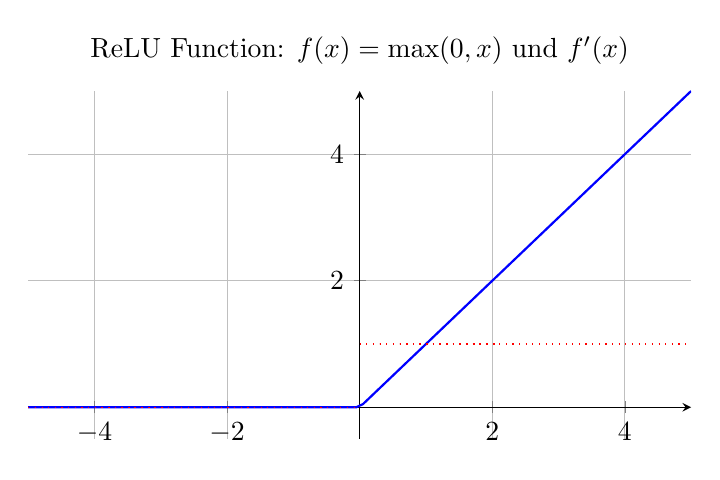
\begin{tikzpicture}
        \begin{axis}[
            axis lines=middle,
            samples=100,
            domain=-5:5,
            width=10cm,
            height=6cm,
            grid=both,
            ymin=-0.5,
            ymax=5,
            title={ReLU Function: $f(x) = \max(0, x)$ und $f'(x)$},
        ]
            \addplot[blue, thick, domain=-5:5] {max(0,x)};

            \addplot[red, dotted, domain=-5:0] {0};
            \addplot[red, dotted, domain=0:5] {1};

        \end{axis}
    \end{tikzpicture}

\end{document}